% ===================================================================
%  Week 8 — Lecture Notes (Persian) — Segmentation
% ===================================================================
\documentclass[12pt,a4paper]{article}
% ===================================================================
%  Shared preamble for Persian lecture notes (Image Processing).
%  Compile with XeLaTeX.  Body = Persian (RTL), code/math = LTR.
% ===================================================================

\usepackage{geometry}
\geometry{a4paper,margin=2.4cm}
\usepackage{amsmath,amssymb}
\usepackage{graphicx}
\usepackage{xcolor}
\usepackage{listings}
\usepackage{tcolorbox}
\usepackage{booktabs}
\usepackage{array}
\usepackage{enumitem}
\usepackage{hyperref}
\tcbuselibrary{skins,breakable}

% ---- Persian / RTL --------------------------------------------------
\usepackage{xepersian}
\settextfont{IRNazli}
\setlatintextfont{Latin Modern Roman}
\setdigitfont{IRNazli}
% More generous leading + paragraph spacing (Persian reads better with air).
\linespread{1.5}
\setlength{\parskip}{0.7em}

% ---- Colours --------------------------------------------------------
\definecolor{coursePrimary}{HTML}{1B4965}
\definecolor{courseAccent}{HTML}{E76F51}
\definecolor{courseGood}{HTML}{2A9D8F}
\definecolor{courseBad}{HTML}{C0392B}
\definecolor{courseInfo}{HTML}{2980B9}
\definecolor{codeBg}{HTML}{F5F6FA}
\definecolor{codeKw}{HTML}{8E44AD}
\definecolor{codeStr}{HTML}{2A9D8F}
\definecolor{codeCom}{HTML}{7F8C8D}

\hypersetup{colorlinks=true,linkcolor=courseInfo,urlcolor=courseInfo,citecolor=courseInfo}

% ---- Code listings (Python built in) -------------------------------
\lstdefinestyle{course}{
  backgroundcolor=\color{codeBg},
  basicstyle=\ttfamily\small,
  keywordstyle=\color{codeKw}\bfseries,
  stringstyle=\color{codeStr},
  commentstyle=\color{codeCom}\itshape,
  numberstyle=\tiny\color{codeCom},
  numbers=left, numbersep=7pt,
  showstringspaces=false, breaklines=true,
  tabsize=4, columns=fullflexible, frame=single,
  rulecolor=\color{gray!30}, keepspaces=true, upquote=true, language=Python,
}
\lstset{style=course}
\lstdefinelanguage{bash}{
  keywords={cd,pip,python,venv,source,import}, sensitive=true,
  morecomment=[l]{\#}, morestring=[b]', morestring=[b]",
}
\newenvironment{ltrcode}{\begin{LTR}}{\end{LTR}}

% ---- Callout boxes (Persian titles) --------------------------------
\newtcolorbox{yaddasht}{colback=courseInfo!8,colframe=courseInfo,
  title={\textbf{یادداشت}},boxrule=0.6pt,right=6pt,left=6pt,breakable}
\newtcolorbox{nokte}{colback=courseAccent!10,colframe=courseAccent,
  title={\textbf{نکتهٔ کلیدی}},boxrule=0.6pt,right=6pt,left=6pt,breakable}
\newtcolorbox{hoshdar}{colback=courseBad!8,colframe=courseBad,
  title={\textbf{هشدار / دام}},boxrule=0.6pt,right=6pt,left=6pt,breakable}
\newtcolorbox{riyazi}{colback=coursePrimary!6,colframe=coursePrimary,
  title={\textbf{ریاضیات}},boxrule=0.6pt,right=6pt,left=6pt,breakable}
\newtcolorbox{tamrin}{colback=courseGood!8,colframe=courseGood,
  title={\textbf{تمرین}},boxrule=0.6pt,right=6pt,left=6pt,breakable}

% ---- Header helper --------------------------------------------------
\newcommand{\coursemeta}[2]{%
  \begin{center}
  {\large\textbf{پردازش تصویرِ کاربردی}}\\[2pt]
  {\color{coursePrimary}\rule{\linewidth}{1pt}}\\[4pt]
  {\Large\textbf{#1}}\\[3pt]
  {\small جزوهٔ درس — #2}
  \end{center}\vspace{4pt}
}


\begin{document}
\coursemeta{جلسهٔ ۸ — قطعه‌بندی}{هفتهٔ هشتم}

{\small\itshape مکملِ اسلایدهای انگلیسیِ جلسهٔ ۸. تصاویر از دیتاستِ واقعیِ شما (کنتور، خودرو) تولید شده‌اند. هدف: تقسیمِ تصویر به نواحیِ معنادار — شیء در برابرِ پس‌زمینه، یا هر شیء جداگانه.}

\vspace{0.5cm}
\tableofcontents
\vspace{1cm}

% ===================================================================
\section{چرا این جلسه}

جلسات ۲ و ۷ آستانه‌گذاری و مورفولوژی را دادند. امروز \textbf{قطعه‌بندی} (\lr{segmentation}) —
افرازِ تصویر به نواحیِ معنادار — را کامل می‌کنیم. برای DocScan: هر رقم را به‌عنوانِ ناحیهٔ خودش
قطعه‌بندی کنید، حتی وقتی دو رقم به هم چسبیده‌اند، تا بتوان یکی‌یکی خواندشان.

\begin{nokte}
قطعه‌بندی جایی است که «پیکسل‌ها» به «اشیا» تبدیل می‌شوند. هر چیزِ پایین‌دستی (شمارش، خواندن) به آن
بستگی دارد. یک قطعه‌بندیِ بد، خواندنِ رقم را غیرممکن می‌کند حتی اگر بقیهٔ خطِ لوله عالی باشد.
\end{nokte}

\subsection{چه چیزی قطعه‌بندی را سخت می‌کند}

قطعه‌بندی یکی از سخت‌ترین مسائلِ بینایی است، به چند دلیل: (۱) \textbf{ابهام} — مرزِ یک شیء کجاست
وقتی سایه یا انعکاس دارد؟ (۲) \textbf{تنوع} — همان شیء زیرِ نورهای مختلف متفاوت به‌نظر می‌رسد؛
(۳) \textbf{اشیای چسبیده} — کجا یکی تمام و دیگری شروع می‌شود؟ (۴) \textbf{بافت} — یک ناحیهٔ
«یکنواخت» ممکن است پیکسل‌های بسیار متفاوت داشته باشد.

برای همین هیچ روشِ واحدی همیشه کار نمی‌کند. هنرِ مهندسی این است که ساختارِ \emph{خاصِ} مسئله را
بشناسید و روشِ متناظر را انتخاب کنید: آیا اشیا با شدت جدا می‌شوند (آستانه)؟ با رنگ (k-means)؟ با
شکل و اتصال (watershed)؟ اغلب \emph{ترکیبی} از روش‌ها لازم است — دقیقاً کاری که خطِ لولهٔ DocScan
می‌کند.

\begin{nokte}
یک بینشِ کلیدی: قطعه‌بندیِ خوب اغلب به \emph{پیش‌پردازشِ} خوب بستگی دارد. اگر تصویر را در جلسات
۲–۷ خوب آماده کرده باشید (کنتراست، حذفِ نویز، مورفولوژی)، قطعه‌بندی بسیار ساده‌تر می‌شود. برعکس،
هیچ روشِ قطعه‌بندیِ هوشمندی نمی‌تواند یک تصویرِ بد‌آماده‌شده را نجات دهد.
\end{nokte}

% ===================================================================
\section{قطعه‌بندی مبتنی بر آستانه}

قطعه‌بندی یعنی به هر پیکسل یک برچسب دادن. ساده‌ترین حالت: دو برچسب (شیء/پس‌زمینه) = آستانه‌گذاری
(جلسهٔ ۲). سخت‌تر: چند شیء، اشیای چسبیده، یا نواحیِ تعریف‌شده با رنگ/بافت.

\begin{center}
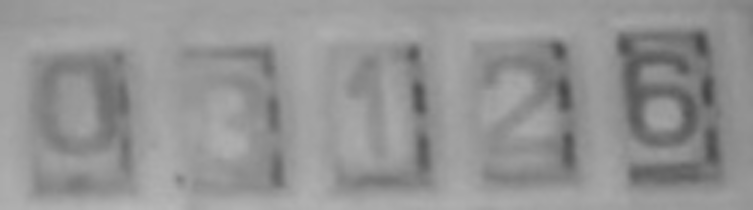
\includegraphics[width=0.31\linewidth]{../assets/gray.png}\quad

\includegraphics[width=0.31\linewidth]{../assets/otsu.png}\quad
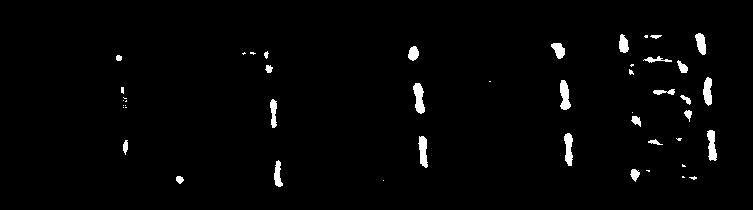
\includegraphics[width=0.31\linewidth]{../assets/adaptive.png}\\[2pt]
{\small چپ: خاکستری — وسط: Otsuِ سراسری — راست: تطبیقی}
\end{center}

Otsu یک آستانهٔ سراسری انتخاب می‌کند (عالی برای نورِ یکنواخت)؛ تطبیقی یک آستانهٔ محلی محاسبه می‌کند
(مقاوم به سایه).

\begin{riyazi}
Otsu آستانهٔ $t$ای را می‌یابد که واریانسِ بین‌کلاسی را بیشینه کند:
$\sigma_B^2(t)=w_0(t)\,w_1(t)\,[\mu_0(t)-\mu_1(t)]^2$
که $w$ نسبتِ هر کلاس و $\mu$ میانگینِ آن است. وقتی هیستوگرام به‌وضوح دوقله‌ای است کار می‌کند.
\end{riyazi}

Otsu شکست می‌خورد روی: نورِ ناهموار، بیش از دو کلاس، یا هیستوگرامِ تک‌قله‌ای.

\subsection{فرض‌های پنهانِ آستانه‌گذاری}

آستانه‌گذاری ساده به‌نظر می‌رسد اما فرض‌های قوی دارد که وقتی نقض شوند شکست می‌خورد: (۱) شیء و
پس‌زمینه \emph{شدت‌های متمایز} دارند؛ (۲) نور \emph{یکنواخت} است؛ (۳) فقط \emph{دو} کلاس هست.
یک عکسِ کنتورِ واقعی اغلب هر سه را نقض می‌کند: ارقام و پس‌زمینه ممکن است شدتِ مشابه داشته باشند،
نور ناهموار است، و انعکاس‌ها کلاسِ سومی می‌سازند.

برای همین آستانه‌گذاری به‌تنهایی به‌ندرت کافی است — معمولاً با پیش‌پردازش (بهبودِ کنتراست، حذفِ
نویز، top-hat برای نور) و پس‌پردازش (مورفولوژی، watershed) ترکیب می‌شود. دانستنِ \emph{فرض‌های}
یک روش، به شما می‌گوید کِی شکست می‌خورد و چه چیزی باید کنارش بگذارید.

% ===================================================================
\section{قطعه‌بندی مبتنی بر ناحیه}

آستانه‌گذاری فقط از شدت استفاده می‌کند؛ روش‌های ناحیه‌ای از \emph{شباهت و اتصال} استفاده می‌کنند —
قدرتمندتر، پارامترِ بیشتر.

\begin{itemize}
  \item \textbf{رشدِ ناحیه} (\lr{region growing}): از دانه‌ها شروع کنید، همسایه‌های به‌قدرِ کافی مشابه را اضافه کنید.
  \item \textbf{تقسیم-و-ادغام} (\lr{split-and-merge}): تصویر را تقسیم کنید، سپس نواحیِ مشابه را ادغام کنید.
  \item \textbf{رنگ/k-means}: پیکسل‌ها را بر اساسِ رنگ به $k$ ناحیه خوشه کنید.
\end{itemize}

\subsection{قطعه‌بندیِ رنگیِ k-means — خودروی واقعی}

\begin{center}
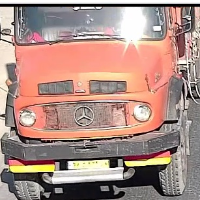
\includegraphics[width=0.4\linewidth]{../assets/car.png}\quad
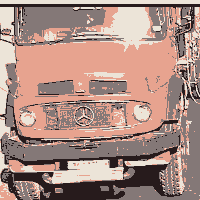
\includegraphics[width=0.4\linewidth]{../assets/car_kmeans.png}\\[2pt]
{\small چپ: اصلی — راست: k-means با $k=4$ رنگ}
\end{center}

هر پیکسل یک نقطه در فضای $(R,G,B)$ است؛ k-means آن‌ها را به $k$ خوشه گروه می‌کند. هر پیکسل را با
رنگِ خوشه‌اش جایگزین کنید $\rightarrow$ یک تصویرِ قطعه‌بندی‌شده و پوستری.

\textbf{الگوریتمِ k-means:} (۱) $k$ مرکزِ اولیه انتخاب کن؛ (۲) هر پیکسل را به نزدیک‌ترین مرکز
تخصیص بده؛ (۳) هر مرکز را میانگینِ پیکسل‌هایش بازمحاسبه کن؛ (۴) تا پایداری تکرار کن.

\textbf{بهبود با موقعیت:} k-meansِ ساده فقط رنگ را می‌بیند، پس دو ناحیهٔ هم‌رنگِ جدا در یک خوشه
می‌افتند. برای رفع این، می‌توان مختصاتِ $(x, y)$ را هم به بردارِ ویژگیِ هر پیکسل اضافه کرد:
$[R, G, B, x, y]$. حالا خوشه‌بندی هم رنگ و هم \emph{مکان} را در نظر می‌گیرد، و نواحیِ پیوسته‌تری
می‌سازد. این ایده پایهٔ الگوریتم‌های \lr{superpixel} (مثلِ SLIC) است که تصویر را به قطعاتِ کوچکِ
منسجم تقسیم می‌کنند.

\begin{yaddasht}
انتخابِ \emph{بردارِ ویژگی} برای هر پیکسل یک تصمیمِ طراحیِ مهم است: فقط شدت؟ رنگ؟ رنگ + موقعیت؟
رنگ + بافت؟ هرچه ویژگی‌های غنی‌تری بدهید، قطعه‌بندیِ معنادارتری می‌گیرید — این پیش‌درآمدِ ایدهٔ
«ویژگی» در جلسات ۱۰ و ۱۲ است.
\end{yaddasht}

\begin{hoshdar}
باید $k$ را انتخاب کنید؛ $k$ی اشتباه بیش/کم‌قطعه‌بندی می‌کند. همچنین \emph{موقعیت} را نادیده
می‌گیرد — فقط رنگ. برای همین دو شیءِ هم‌رنگ در جاهای مختلف در یک خوشه می‌افتند.
\end{hoshdar}

% ===================================================================
\section{Watershed: جدا کردنِ اشیای چسبیده}

آستانه + مورفولوژی لکه‌ها می‌دهد — اما دو رقمِ چسبیده یک لکهٔ \emph{واحد} می‌شوند. شمارش/خواندن به
جداییِ آن‌ها نیاز دارد. فرسایش کمی کمک می‌کند اما می‌تواند ضربه‌های نازک را بشکند. \textbf{Watershed}
این را درست حل می‌کند، با استفاده از شکل (یک تبدیلِ فاصله).

\begin{center}

\includegraphics[width=0.44\linewidth]{../assets/distance.png}\quad
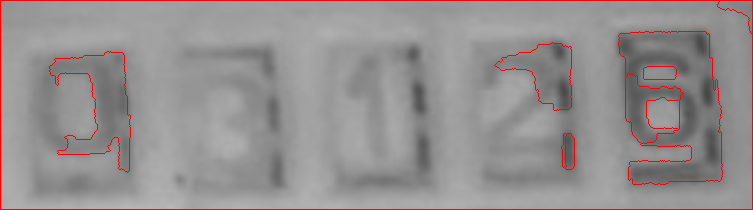
\includegraphics[width=0.44\linewidth]{../assets/watershed.png}\\[2pt]
{\small چپ: تبدیلِ فاصله — راست: مرزهای watershed (قرمز)}
\end{center}

\textbf{تبدیلِ فاصله} (\lr{distance transform}) در مرکزِ هر شیء پیک می‌زند؛ watershed از آن پیک‌ها
«سیل» می‌کند و جایی که سیل‌ها به‌هم می‌رسند یک ستیغ می‌سازد — مرزِ جداکننده.

\subsection{تبدیلِ فاصله با جزئیات}

\textbf{تبدیلِ فاصله} برای هر پیکسلِ پیش‌زمینه، فاصله‌اش تا نزدیک‌ترین پیکسلِ پس‌زمینه را محاسبه
می‌کند. نتیجه: پیکسل‌های مرکزیِ یک شیء (که دورترین از لبه‌اند) بالاترین مقدار را دارند، و لبه‌ها
مقدارِ نزدیکِ صفر. پس تبدیلِ فاصله، «کوه»ی می‌سازد که قله‌اش مرکزِ هر شیء است.

چرا این برای watershed کلیدی است؟ چون قله‌های تبدیلِ فاصله، \emph{نشانگرهای} طبیعیِ مراکزِ اشیا
هستند. با آستانه‌گذاریِ تبدیلِ فاصله (مثلاً بالای ۵۰٪ بیشینه)، مراکزِ قطعیِ اشیا را می‌یابید — حتی
برای دو رقمِ چسبیده، دو قلهٔ جدا وجود دارد. این ترکیبِ «تبدیلِ فاصله + watershed» یکی از قوی‌ترین
تکنیک‌های جدا کردنِ اشیای چسبیده در پردازشِ تصویرِ کلاسیک است.

\begin{riyazi}
تبدیلِ فاصلهٔ اقلیدسی: $D(p) = \min_{q \in \text{background}} \|p - q\|$. \lr{OpenCV} این را با
\lr{cv2.DIST\_L2} به‌طورِ کارآمد محاسبه می‌کند.
\end{riyazi}

\subsection{شهودِ watershed}

شدت (یا منفیِ فاصله) را یک منظره در نظر بگیرید؛ «آب» از کمینه‌های علامت‌دار بالا می‌آید. جایی که
دو حوضه به هم می‌رسند، یک سد بسازید — آن سد مرزِ شیء است. \textbf{نشانگرها} (\lr{markers}) آن را
کنترل می‌کنند، وگرنه \emph{بیش‌قطعه‌بندی} می‌کند (هر کمینهٔ ریز یک ناحیه). watershedِ کنترل‌شده با
نشانگر نسخهٔ قابلِ‌اعتماد است: پیش‌زمینه و پس‌زمینهٔ قطعی را به آن می‌گویید.

\begin{ltrcode}
\begin{lstlisting}[language=Python]
dist = cv2.distanceTransform(binary, cv2.DIST_L2, 5)
_, sure_fg = cv2.threshold(dist, 0.5*dist.max(), 255, 0)   # digit centres
sure_bg = cv2.dilate(binary, k, iterations=3)
unknown = cv2.subtract(sure_bg, np.uint8(sure_fg))
_, markers = cv2.connectedComponents(np.uint8(sure_fg))
markers = markers + 1; markers[unknown==255] = 0
markers = cv2.watershed(color_img, markers)               # -1 = boundaries
\end{lstlisting}
\end{ltrcode}

% ===================================================================
\section{مؤلفه‌های همبند}

\begin{center}

\includegraphics[width=0.6\linewidth]{../assets/components.png}\\[2pt]
{\small هر لکه با یک رنگِ متفاوت — مؤلفه‌های همبند}
\end{center}

\textbf{مؤلفه‌های همبند} (\lr{connected components}) هر ناحیهٔ سفیدِ جدا را با یک عددِ صحیح برچسب
می‌زند. پس از جداسازی، هر رقم مؤلفهٔ خودش است که می‌توانید برشش دهید و بخوانید (جلسهٔ ۹).
\lr{cv2.connectedComponentsWithStats} برچسب‌ها + مساحت + کادرها را می‌دهد.

\begin{nokte}
اتصال دو نوع دارد: ۴-همبندی (فقط بالا/پایین/چپ/راست) و ۸-همبندی (شاملِ قطرها). انتخابِ آن بر
تعدادِ مؤلفه‌ها اثر می‌گذارد: با ۸-همبندی، اشیایی که فقط از گوشه به هم می‌رسند یک مؤلفه می‌شوند.
\end{nokte}

% ===================================================================
\section{رشدِ ناحیه با جزئیات}

\textbf{رشدِ ناحیه} یک روشِ شهودی است: از یک یا چند \emph{دانه} (\lr{seed}) شروع کنید، و به‌طورِ
مکرر پیکسل‌های همسایه‌ای را که با ناحیه به‌قدرِ کافی «شبیه»‌اند (مثلاً اختلافِ شدتشان از میانگینِ
ناحیه کمتر از یک آستانه است) اضافه کنید. ناحیه رشد می‌کند تا دیگر همسایهٔ مشابهی نماند.

\textbf{مزیت}: از \emph{اتصال} استفاده می‌کند، پس دو ناحیهٔ هم‌شدتِ جدا را قاطی نمی‌کند (برخلافِ
آستانهٔ سراسری). \textbf{ضعف}: به انتخابِ دانه و آستانهٔ شباهت حساس است؛ دانهٔ بد یا آستانهٔ بزرگ،
باعثِ «نشتِ» ناحیه به بیرون می‌شود.

\begin{nokte}
رشدِ ناحیه پلی بین آستانه‌گذاری (فقط شدت) و watershed (شکل + اتصال) است. برای اشیایی با شدتِ
نسبتاً یکنواخت اما پس‌زمینهٔ پیچیده مفید است. در عمل، اغلب watershed یا روش‌های مدرن جایگزینش
می‌شوند، اما شهودِ «از دانه رشد کن» در بسیاری الگوریتم‌ها تکرار می‌شود.
\end{nokte}

% ===================================================================
\section{بیش‌قطعه‌بندیِ watershed}

مشکلِ اصلیِ watershedِ خام: \textbf{بیش‌قطعه‌بندی} (\lr{over-segmentation}). چون هر کمینهٔ محلیِ
منظره یک حوضه می‌سازد، نویز و بافتِ ریز ده‌ها ناحیهٔ کاذب ایجاد می‌کنند. راه‌حل‌ها:

\begin{itemize}
  \item \textbf{کنترل با نشانگر}: فقط از کمینه‌های \emph{انتخاب‌شده} (پیش‌زمینهٔ قطعی) سیل کنید، نه همهٔ کمینه‌ها.
  \item \textbf{هموارسازیِ اولیه}: تصویر را اول تار کنید تا کمینه‌های نویزی حذف شوند.
  \item \textbf{ادغامِ بعدی}: نواحیِ کوچکِ مجاور را پس از watershed ادغام کنید.
\end{itemize}

\begin{hoshdar}
watershedِ بدونِ نشانگر تقریباً همیشه بیش‌قطعه‌بندی می‌کند و بی‌فایده است. همیشه نسخهٔ
کنترل‌شده‌با‌نشانگر را استفاده کنید — تبدیلِ فاصله + آستانه برای یافتنِ مراکزِ قطعیِ اشیا، همان
کاری که در کد کردیم.
\end{hoshdar}

% ===================================================================
\section{انواعِ آستانه و کِی هرکدام}

\begin{center}
\begin{tabular}{>{\raggedright\arraybackslash}p{0.3\linewidth} >{\raggedright\arraybackslash}p{0.6\linewidth}}
\toprule
\textbf{روش} & \textbf{کِی} \\
\midrule
آستانهٔ ثابت & نور کنترل‌شده، آستانهٔ معلوم \\
Otsu & نورِ یکنواخت، هیستوگرامِ دوقله‌ای \\
تطبیقی & نورِ ناهموار، سایه \\
آستانهٔ رنگی (HSV) & شیء با رنگِ متمایز \\
چند-آستانه (multi-Otsu) & بیش از دو کلاس (مثلاً پس‌زمینه/متن/های‌لایت) \\
\bottomrule
\end{tabular}
\end{center}

\begin{yaddasht}
یک تعمیمِ مفید: \textbf{Otsu چند‌سطحی} (\lr{multi-Otsu}) می‌تواند بیش از یک آستانه بیابد و تصویر
را به چند کلاس تقسیم کند — مثلاً پس‌زمینهٔ روشن، متنِ خاکستری، و لکه‌های تیره. برای اسنادِ پیچیده مفید است.
\end{yaddasht}

% ===================================================================
\section{تمرینِ کلاسیِ وسط‌جلسه (۱۲ دقیقه)}

\begin{tamrin}
کدام روشِ قطعه‌بندی مناسبِ هر تسک است؟ (۱) جدا کردنِ متنِ تیره از صفحهٔ روشن با نورِ یکنواخت. (۲)
دو رقمِ کنتور که چسبیده‌اند و باید جدا شمرده شوند. (۳) قطعه‌بندیِ عکس به نواحیِ «آسمان/جاده/خودرو»
با رنگ. (۴) سندی که با سایه‌ای روی نیمی از آن عکس گرفته شده.
\end{tamrin}

\textbf{جمع‌بندی:} (۱) نورِ یکنواخت، دوقله‌ای $\rightarrow$ \textbf{Otsu}. (۲) اشیای چسبیده
$\rightarrow$ \textbf{watershed}. (۳) نواحیِ رنگی $\rightarrow$ \textbf{k-means} (یا آستانهٔ
رنگی در HSV). (۴) سایه $\rightarrow$ آستانهٔ \textbf{تطبیقی} (محلی)، نه Otsuِ سراسری. هیچ روشِ
واحدی برنده نیست؛ روش را با ساختار تطبیق دهید: شدت، رنگ، اتصال، یا نور.

% ===================================================================
\section{بخشِ عمیق}

\subsection{ارزیابیِ یک قطعه‌بندی}

با ماسک‌های حقیقتِ زمینه: \textbf{IoU} (اشتراک بر اجتماع) و امتیازِ \textbf{Dice}. بیش‌قطعه‌بندی
(نواحیِ خیلی زیاد) در برابرِ کم‌قطعه‌بندی (نواحیِ ادغام‌شده) — هر دو خطا هستند. برای DocScan، آزمونِ
واقعی پایین‌دستی است: آیا هر رقم پس از قطعه‌بندی خوانده می‌شود؟

\begin{riyazi}
$\mathrm{IoU}=\dfrac{|A\cap B|}{|A\cup B|}$، $\mathrm{Dice}=\dfrac{2|A\cap B|}{|A|+|B|}$؛
مقدارِ ۱٫۰ هم‌پوشانیِ کامل با حقیقت است.
\end{riyazi}

\subsection{مثالِ عددیِ IoU}

فرض کنید ماسکِ پیش‌بینیِ ما ۱۰۰ پیکسل دارد، ماسکِ حقیقت ۱۲۰ پیکسل، و ۸۰ پیکسل مشترک‌اند. آنگاه:
\[
|A \cap B| = 80, \quad |A \cup B| = 100 + 120 - 80 = 140
\]
\[
\mathrm{IoU} = \frac{80}{140} \approx 0.57, \qquad \mathrm{Dice} = \frac{2 \times 80}{100 + 120} \approx 0.73
\]
Dice همیشه از IoU بزرگ‌تر یا مساوی است. IoUِ ۰٫۵ معمولاً «قابلِ‌قبول» و بالای ۰٫۷ «خوب» تلقی
می‌شود. این اعداد به شما اجازه می‌دهند دو روشِ قطعه‌بندی را \emph{عینی} مقایسه کنید، به‌جای قضاوتِ چشمی.

\subsection{قطعه‌بندیِ معنایی در برابرِ نمونه‌ای}

دو نوعِ قطعه‌بندیِ مدرن که در جلسات ۱۳–۱۴ می‌بینیم: \textbf{معنایی} (\lr{semantic}) هر پیکسل را
به یک \emph{کلاس} برچسب می‌زند (همهٔ خودروها «خودرو») اما نمونه‌ها را جدا نمی‌کند. \textbf{نمونه‌ای}
(\lr{instance}) هر شیءِ جداگانه را هم متمایز می‌کند (خودروی ۱، خودروی ۲). برای شمارشِ ارقام،
قطعه‌بندیِ \emph{نمونه‌ای} می‌خواهیم — هر رقم جدا. watershed در واقع یک روشِ کلاسیکِ قطعه‌بندیِ
نمونه‌ای است.

\begin{yaddasht}
درکِ این تمایز مهم است: اگر فقط بپرسید «کدام پیکسل‌ها رقم‌اند؟» یک ماسکِ معنایی کافی است؛ اما اگر
بخواهید «چند رقم و هرکدام چیست؟»، به قطعه‌بندیِ نمونه‌ای نیاز دارید که ارقام را از هم جدا کند.
\end{yaddasht}

\subsection{کلاسیک در برابرِ عمیق}

کلاسیک (آستانه/watershed/k-means): سریع، قابلِ‌تفسیر، بدونِ آموزش — عالی برای تصاویرِ تمیز و
ساختارمند. عمیق (\lr{U-Net}، \lr{Mask R-CNN}، \lr{SAM}): یاد می‌گیرد صحنه‌های پیچیده را قطعه‌بندی
کند، اما به داده/محاسبه نیاز دارد. برای کنتور/سند، کلاسیک اغلب کافی است؛ عمیق در صحنه‌های طبیعیِ
درهم می‌درخشد (جلسات ۱۳–۱۴).

\subsection{GrabCut و روش‌های مبتنی بر گراف}

\textbf{GrabCut} توزیعِ رنگِ پیش/پس‌زمینه را مدل و گراف را بهینه برش می‌زند — برشِ شیءِ تعاملی.
روش‌های \lr{graph-cut}/\lr{normalized-cut}، قطعه‌بندی را افرازِ یک گرافِ پیکسلی می‌بینند: هر پیکسل
یک گره، و شباهتِ همسایه‌ها وزنِ یال. یک «برشِ» بهینه، گراف را به دو بخش (شیء/پس‌زمینه) تقسیم می‌کند
که کمترین شباهت را قطع کند. این‌ها پلِ بینِ کلاسیک و مدرن‌اند.

قطعه‌بندیِ \textbf{تعاملی} یک ایدهٔ عملیِ قدرتمند است: کاربر چند خط روی پیش‌زمینه و پس‌زمینه می‌کشد،
و الگوریتم بقیه را استنتاج می‌کند. این تعادلِ خوبی بین کارِ دستیِ کامل و خودکارسازیِ کامل است — و
در ابزارهای واقعیِ ویرایشِ تصویر (مثلِ «انتخابِ هوشمند») رایج است. مدل‌های مدرنی مثلِ \lr{SAM}
(\lr{Segment Anything}) این را به سطحِ جدیدی برده‌اند: با یک کلیک، هر شیء را قطعه‌بندی می‌کنند.

\begin{yaddasht}
پیامِ کلی: قطعه‌بندی طیفی از «کاملاً خودکار» تا «کاملاً دستی» دارد. برای یک کنتورِ ساختارمند،
خودکارِ کلاسیک کافی است؛ برای یک صحنهٔ پیچیده، ترکیبِ تعاملی یا مدلِ عمیق. انتخابِ نقطهٔ درست روی
این طیف، بخشی از مهندسیِ راه‌حل است.
\end{yaddasht}

% ===================================================================
\section{این جلسه در پروژهٔ نهایی}

خطِ لولهٔ قطعه‌بندیِ DocScan: آستانه $\rightarrow$ مورفولوژی $\rightarrow$ watershed (جدا کردنِ
ارقامِ چسبیده) $\rightarrow$ مؤلفه‌ها (برچسب‌زدنِ هر رقم) $\rightarrow$ خواندن (جلسهٔ ۱۳). هر رقم به
یک تصویرِ منزوی تبدیل می‌شود که CNN می‌تواند دسته‌بندی کند.

\begin{yaddasht}
\textbf{مایلستونِ هفتهٔ ۸:} از یک عکسِ کنتور، یک تصویرِ برش‌خورده به‌ازای هر رقم تولید کنید، به
ترتیبِ چپ‌به‌راست. اگر ارقام می‌چسبند، watershed لازم است. این خروجی مستقیماً ورودیِ شناساییِ
جلسهٔ ۱۳ است — پس ترتیب و تمیزیِ برش‌ها حیاتی است.
\end{yaddasht}

\subsection{ترکیبِ روش‌ها — یک خطِ لولهٔ واقعی}

در عمل، یک قطعه‌بندیِ خوب اغلب زنجیره‌ای از روش‌هاست. برای جدا کردنِ ارقامِ یک کنتور:

\begin{ltrcode}
\begin{lstlisting}[language=Python]
# 1. threshold (Week 2)
_, b = cv2.threshold(gray, 0, 255, cv2.THRESH_BINARY_INV + cv2.THRESH_OTSU)
# 2. clean with morphology (Week 7)
b = cv2.morphologyEx(b, cv2.MORPH_OPEN, k)
# 3. separate touching digits with distance + watershed (this week)
dist = cv2.distanceTransform(b, cv2.DIST_L2, 5)
# ... watershed markers ...
# 4. label each digit and sort left-to-right
n, lbl, stats, cent = cv2.connectedComponentsWithStats(b)
boxes = sorted(stats[1:], key=lambda s: s[0])   # sort by x
digits = [gray[y:y+h, x:x+w] for x, y, w, h, area in boxes]
\end{lstlisting}
\end{ltrcode}

هر گام ورودیِ گامِ بعد را آماده می‌کند. هیچ روشِ واحدی نمی‌توانست همهٔ این را انجام دهد — قدرت در
\emph{ترکیب} است. این دقیقاً فلسفهٔ کلِ کورس است: جعبه‌ابزاری از تکنیک‌های ساده که به سیستم‌های
قدرتمند ترکیب می‌شوند.

\subsection{مرتب‌سازیِ ارقام}

یک نکتهٔ عملی: پس از یافتنِ مؤلفه‌ها، باید آن‌ها را \emph{مرتب} کنید (چپ‌به‌راست) تا عددِ درست
بازسازی شود. کادرِ هر مؤلفه را بگیرید و بر اساسِ مختصاتِ $x$ مرتب کنید. بدونِ این، ارقام را درست
می‌خوانید اما به ترتیبِ غلط — و «۳۶۷۹» می‌شود «۷۳۹۶».

% ===================================================================
\section{جمع‌بندی}

\begin{itemize}
  \item قطعه‌بندی با آستانه (سراسری/تطبیقی/Otsu) و دانستنِ اینکه کدام کِی شکست می‌خورد.
  \item استفاده از k-means برای قطعه‌بندیِ رنگی؛ روش‌های ناحیه‌ای برای شباهت.
  \item جدا کردنِ اشیای چسبیده با watershedِ کنترل‌شده با نشانگر.
  \item برچسب‌زدنِ لکه‌ها با مؤلفه‌های همبند؛ ارزیابی با IoU/Dice.
\end{itemize}

\begin{tamrin}
\textbf{تحویلیِ این هفته (پیش از جلسهٔ ۹):} (۱) Otsu و تطبیقی را روی تصاویرِ کنتور مقایسه کنید؛
برندهٔ هر نور را انتخاب کنید. (۲) قطعه‌بندیِ رنگیِ k-means روی یک خودرو/پلاک با $k=2,4,8$؛ بحث
کنید. (۳) watershed برای جدا کردنِ ارقامِ چسبیده؛ هرکدام را با مؤلفه‌های همبند برچسب بزنید. (۴)
مایلستونِ DocScan: یک تصویرِ برش‌خورده به‌ازای هر رقم، به ترتیب.
\end{tamrin}

\subsection*{کاربردهای قطعه‌بندی}

\begin{itemize}
  \item \textbf{OCR/خواندنِ کنتور}: جدا کردنِ هر رقم/کاراکتر (DocScan).
  \item \textbf{پزشکی}: قطعه‌بندیِ تومور، اندام، سلول در MRI/میکروسکوپ.
  \item \textbf{صنعتی}: جدا کردن و شمارشِ قطعات؛ تشخیصِ عیب.
  \item \textbf{کشاورزی}: قطعه‌بندیِ برگ/میوه در تصویرِ هوایی.
  \item \textbf{خودران}: جدا کردنِ جاده، عابر، خودرو (قطعه‌بندیِ معنایی).
\end{itemize}

\subsection*{چک‌لیستِ دام‌های این هفته}

\begin{itemize}
  \item Otsuِ سراسری روی نورِ ناهموار — به‌جایش تطبیقی.
  \item watershed بدونِ نشانگر (بیش‌قطعه‌بندی) — نسخهٔ کنترل‌شده.
  \item $k$ی اشتباه در k-means (بیش/کم‌قطعه‌بندی) — چند $k$ را امتحان کنید.
  \item فراموشیِ مرتب‌سازیِ ارقام پس از یافتنِ مؤلفه‌ها — ترتیبِ غلطِ عدد.
  \item ارزیابیِ چشمی به‌جای IoU/Dice یا آزمونِ پایین‌دستی.
\end{itemize}

\subsection*{واژه‌نامهٔ کوتاه}

\begin{center}
\begin{tabular}{>{\raggedright\arraybackslash}p{0.3\linewidth} >{\raggedright\arraybackslash}p{0.6\linewidth}}
\toprule
\textbf{اصطلاح} & \textbf{معنی} \\
\midrule
\lr{Segmentation} & افرازِ تصویر به نواحیِ معنادار \\
\lr{Otsu / Adaptive} & انتخابِ آستانهٔ سراسری / محلی \\
\lr{k-means} & خوشه‌بندیِ پیکسل‌ها (رنگ) به $k$ ناحیه \\
\lr{Watershed} & جدا کردنِ اشیای چسبیده با سیل از نشانگرها \\
\lr{Distance transform} & فاصلهٔ هر پیکسل تا نزدیک‌ترین پس‌زمینه \\
\lr{Connected components} & برچسب‌زدنِ نواحیِ جدا \\
\lr{IoU / Dice} & معیارهای کیفیتِ قطعه‌بندی \\
\bottomrule
\end{tabular}
\end{center}

\vspace{0.5cm}
\begin{center}
\textit{قطعه‌بندی پیکسل‌ها را به اشیا تبدیل می‌کند. آستانه برای دو کلاس، k-means برای رنگ، watershed برای اشیای چسبیده.}
\end{center}

\end{document}
